% Exam Template for UMTYMP and Math Department courses
%
% Using Philip Hirschhorn's exam.cls: http://www-math.mit.edu/~psh/#ExamCls
%
% run pdflatex on a finished exam at least three times to do the grading table on front page.
%
%%%%%%%%%%%%%%%%%%%%%%%%%%%%%%%%%%%%%%%%%%%%%%%%%%%%%%%%%%%%%%%%%%%%%%%%%%%%%%%%%%%%%%%%%%%%%%

% These lines can probably stay unchanged, although you can remove the last
% two packages if you're not making pictures with tikz.
\documentclass[11pt]{exam}
\RequirePackage{amssymb, amsfonts, amsmath, latexsym, xspace, setspace}
\RequirePackage{tikz, pgflibraryplotmarks}

% By default LaTeX uses large margins.  This doesn't work well on exams; problems
% end up in the "middle" of the page, reducing the amount of space for students
% to work on them.
\usepackage[margin=1in]{geometry}
\usepackage{verbatim}

% Here's where you edit the Class, Exam, Date, etc.
\newcommand{\class}{Principles of Operating Systems}
\newcommand{\term}{Fall 2017}
\newcommand{\examnum}{Final}
\newcommand{\examdate}{12/13/2017}
\newcommand{\timelimit}{8:00am - 10:00am}

% For an exam, single spacing is most appropriate
\singlespacing
% \onehalfspacing
% \doublespacing

% For an exam, we generally want to turn off paragraph indentation
\parindent 0ex

\def\answers{1}


\begin{document} 

% These commands set up the running header on the top of the exam pages
\pagestyle{head}
\firstpageheader{}{}{}
\runningheader{\class}{\examnum\ - Page \thepage\ of \numpages}{\examdate}
\runningheadrule

\begin{flushright}
\begin{tabular}{p{2.8in} r l}
\textbf{\class} & \textbf{Name (Print):} & \makebox[2in]{\hrulefill}\\
\textbf{\term} &&\\
\textbf{\examnum} &&\\
\textbf{\examdate} &&\\
\textbf{Time Limit: \timelimit} & & \\
\end{tabular}\\
\end{flushright}
\rule[1ex]{\textwidth}{.1pt}




%\begin{minipage}[t]{3.7in}
%\vspace{0pt}
\begin{itemize}

\item \textbf{Don't forget to write your name on this exam.} 

\item \textbf{This is an open book, open notes exam. But no online or 
    in-class chatting.  } 

    
\item \textbf{Ask me if something is not clear in the questions.}

\item \textbf{Organize your work}, in a reasonably neat and coherent way, in
the space provided. Work scattered all over the page without a clear ordering will 
receive very little credit.  

\item \textbf{Mysterious or unsupported answers will not receive full
credit}.  A correct answer, unsupported by explanation will receive no credit; 
an incorrect answer supported by substantially correct explanations might still 
receive partial credit.

\item If you need more space, use the back of the pages; clearly indicate when you have done this.
\end{itemize}

%Do not write in the table to the right.
%\end{minipage}
%\hfill

%\begin{minipage}[t]{2.3in}
%\vspace{0pt}
%\cellwidth{3em}
%\gradetablestretch{2}
\vqword{Problem}
\addpoints % required here by exam.cls, even though questions haven't started yet.	
\gradetable[v]%[pages]  % Use [pages] to have grading table by page instead of question

%\end{minipage}
\newpage % End of cover page

%%%%%%%%%%%%%%%%%%%%%%%%%%%%%%%%%%%%%%%%%%%%%%%%%%%%%%%%%%%%%%%%%%%%%%%%%%%%%%%%%%%%%
%
% See http://www-math.mit.edu/~psh/#ExamCls for full documentation, but the questions
% below give an idea of how to write questions [with parts] and have the points
% tracked automatically on the cover page.
%
%
%%%%%%%%%%%%%%%%%%%%%%%%%%%%%%%%%%%%%%%%%%%%%%%%%%%%%%%%%%%%%%%%%%%%%%%%%%%%%%%%%%%%%

\begin{questions}

% Basic question
\addpoints
\question File system


Xv6 lays out the file system on disk as follows:

\begin{figure}[h] \centering
  \includegraphics[width=0.8\columnwidth]{figs/fs}
  \label{fig:ramengine-decomposed-app}

\end{figure}

Block 1 contains the super block. Blocks 2 through 31 contain the log header
and the log. Blocks 32 through 57 contain inodes. Block 58 contains the bitmap
of free blocks. Blocks 59 through the end of the disk contain data blocks.

Ben modifies the function bwrite in bio.c to print the block number of each
block written.

Ben boots xv6 with a fresh fs.img and types in the
command rm README, which deletes the README file.
This command produces the following trace:

\begin{verbatim} 
$ rm README
write 3
write 4
write 5
write 2
write 59
write 32
write 58
write 2
$
\end{verbatim}

\begin{parts} 


\part[5] Briefly explain what block 59 contains in the above trace. Why is it written?

\if\answers1

Block 59 contains the data for the ``/'' directory inode. Since Ben delets the file from the ``/'' the directory inode is updated. 

\fi

\vfill

%\newpage

\part[5] What does block 5 contain? Why is it written?

\if\answers1

Block 5 contains the copy of block 58 in the log. Xv6 file system frist writes the log to ensure atomicity of all file system updates, then it copies the log to the actual data blocks. 

\fi

\vfill

\newpage

\part[10] How many non-zero bytes are written to block 2 when it's written the
first time and what are the bytes? (To get the full credit you have to explain
what block 2 contains, and why each non-zero byte is written).   

\if\answers1

Block 2 contains the header of the log, or more specifically an integer (4 bytes) that contains the size of the log, and then an array of integers (4 bytes each) of size LOGSIZE that keep the actual block numbers for the blocks in the log. The log header data structure that is written to block 2 is defined as:

\begin{verbatim}
// Contents of the header block, used for both the on-disk header block
// and to keep track in memory of logged block# before commit.
struct logheader {
  int n;
  int block[LOGSIZE];
};
\end{verbatim}

In our example, n is equal to 3, an then 3 integers are 3, 4, and 5. The total of 4 integers or 16 non-zero bytes are written to block 2. 

If you want to be extra pedantic you can reason about non-zero integers that might be in the block array from previous log transactions. In practice, on a clean xv6 file system, the only one transaction that happened before wrote 2 blocks creating the console device. So the rest of the array is clean anyway. 
 
\vfill
\fi

\end{parts}


%\newpage
\addpoints
\question Synchronization

\begin{parts}

\part[5] Ben runs xv6 on a single CPU machine, he decides it's a good idea to
get rid of the acquire() and release() functions, since after all they take
some time but seem unnecessary in a single-CPU scenario.  Explain if removal of
these functions is fine. 

\if\answers1

No. In addition to acquire a spinlock to enter a critical section, \texttt{acquire()} disables interrupts to prevent an interrupt from entering the critical section and changing one of the protected data strutures concurrently with the process and other interrupts. 

\fi


\vfill

\end{parts}

\newpage
\addpoints
\question Process memory layout

Bob decides to implement the following xv6 program (hello)
\begin{verbatim}
#define PGSIZE  4096
int main(int argc, char *argv[]) {
  char buf[PGSIZE] = {0};
  printf(1, "Hello World!, %p\n", buf);
  exit();
}
\end{verbatim}

\begin{parts}
\part[10] When Bob runs it he encounters the following error message:
  \begin{verbatim}
  pid 3 hello: trap 14 err 7 on cpu 1 eip 0x22 addr 0x1fd0--kill proc
  \end{verbatim}

  Can you help Bob understand the problem? (To receive full points, you
  should explain why this error happened, what does the error values mean and
  how Bob can fix his code)

\if\answers1

Bob allocates an array of 4096 bytes on the stack 

\begin{verbatim}

char buf[PGSIZE] = {0};

\end{verbatim}


\texttt{Buf} is a local variable. It is allocated on the stack. Since xv6 stack is only
one page (4096 bytes), and main already has 47 bytes on the stack
(0x1fff-0x1fd0), the code tries to access the first element of the buffer when the compiler 
generates the code that initializes \texttt{buf} with zeroes. The first element of 
the buffer is actually on the guard page (0x1fd0).  Hence, Bob's
code triggers an exception and xv6 kills the process reporting a violation. 

\fi

  \vfill

\end{parts}

\newpage
\addpoints
\question Virtual memory

Ben wants to know the address of physical pages that back up virtual memory of
his process. He digs into the kernel source and comes across the V2P() macro
that is frequently used in the kernel.

\begin{verbatim}
#define KERNBASE  0x80000000 
#define V2P(a) (((uint) (a)) - KERNBASE)
\end{verbatim}

He decides to try the V2P macro in his program (below), but encounters a crash.
\begin{verbatim}
void test(void) {
  int a;
  *(uint*)V2P(&a) = 0xaddb;
  printf(1, "I changed physical memory at %x\n", a);
}
int main(int argc, char *argv[]) {
  test();
  exit();
}
\end{verbatim}

\begin{parts}
  \part[5] Explain what is going on and why Ben's program crashes. 
  \vfill

\if\answers1 

\fi

  \part[5] Ben puts the code of the test() function inside a new system call trying to see if it works inside the kernel. Will it work (explain your answer)? 
  \vfill

\end{parts}

\newpage
\addpoints
\question Demand paging 

Ben wants to extend xv6 with demand paging. Ben observes that some pages of
user processes (heap, text, and stack) are not accessed
that frequently, yet anyway they consume valuable physical memory. So Ben comes
up with a plan to free these infrequently used pages by saving them to disk (swapping). For an idle page he plans to unmap
it from the process page table, save content of the page to disk (i.e., in a special swap area on disk), and free the physical page back to the 
kernel, making it accessible for other processes. Obviously,
Ben wants paging to be transparent. I.e., when a process accesses one of the
swapped pages, Ben plans to catch an exception, allocate a new physical page,
read old content of the page from disk, and fix the process page table in such a
way that process can access the page like nothing happened. 


%Ben thinks he can catch a virtual memory translation exception, read the page
%from disk, by catching the exception in the xv6 trap handler. 

\begin{parts} 

  \part[5] How can Ben unmap a page from the process address space? I.e., what changes to the process page table are required to catch an exception when the process tries to access a swapped page (hint: look at how guard page is implemented)? 

 \vfill

\newpage
  \part[10] Ben plans to catch the exception caused by an unmapped page access inside the trap() function. Provide a sketch for the code that implements the exception handling, reads page from disk, and maps it back into the process address space. 

  \vfill

\end{parts}

\newpage
\addpoints
\question System call API

Alice 
%
%was reading the fork.c on the IDE and her cat suddenly jumped on the keyboard
%that changed the line 204 from 
%\begin{verbatim}
%203   // Clear %eax so that fork returns 0 in the child.
%204   np->tf->eax = 0;
%\end{verbatim}
%to
%\begin{verbatim}
%203   // Clear %eax so that fork returns 0 in the child.
%204   np->tf->eax = 1;
%\end{verbatim}
%
executes the following program
\begin{verbatim}
main() {
  char *msg = "bar\n";
  int pid = fork();
  if (pid)
    msg = "foo\n";
  else
    msg = "baz\n";
  write(1, msg, 4);
  exit(0);
}
\end{verbatim}

\begin{parts}
  \part[5] What are all possible outputs of this program? Explain your answer.
  \vfill

\end{parts}

%\newpage
\addpoints
\question Process creation
While editing the xv6 code, Jimmy accidentally erases the below section of
code under fork() function on proc.c
\begin{verbatim}
2584 for(i = 0; i < NOFILE; i++)
2585    if(proc->ofile[i])
2586        np->ofile[i] = filedup(proc->ofile[i]);
\end{verbatim}

\begin{parts}
\part[5] Explain what the above section of code does?

  \vfill
\newpage
\part[5] Explain what can go wrong without this piece of code? Quote a concrete example and explain
  the incorrect behavior.
  \vfill
\end{parts}

\newpage
\addpoints

\question cs143A. I would like to hear your opinions about cs143A, so please answer the following questions. (Any answer, except
no answer, will receive full credit.)


\begin{parts}

\part[1] Grade cs143A on a scale of 0 (worst) to 10 (best)?

\vfill

\part[2] Any suggestions for how to improve cs143A?

\vfill

\part[1] What is the best aspect of cs143A?

\vfill

\part[1] What is the worst aspect of cs143A?

\vfill

\end{parts}

\iffalse

\newpage
\addpoints
\question You are given a task of porting xv6 on the hardware that is identical 
to x86, but does not have a paging mechanism. 

\begin{parts}
\part[10] How will you implement address spaces? Remember that address spaces 
provide two key properties: illusion of a private memory, and isolation. Draw a 
figure of an address space layout for 2 processes and the kernel. Provide 
discussion of the mechanisms involved into your implementation.  

\vfill
\part[10] Remember that user processes on xv6 have only one interface to change 
their memory allocation---the \texttt{sbrk(n)} system call that allows the 
process to change its memory allocation growing it by n bytes (or shrinking it 
if a negative value is provided). How will you support \texttt{sbrk()} in your 
xv6 port? What are the data structures required? Provide a design discussion. 

\vfill
\newpage
\part[10] What if two processes want to share a region of memory? Can you 
suggest an interface and implementation for your port? What are the limitations 
of this mechanism, e.g. how many processes can share a region of memory 
simultaneously, how many sharing regions can be established? 

\vfill
\part[10] Discuss advantages and disadvantages of giving up the paging 
mechanism. 


\vfill
\end{parts}

\fi

% If you want the total number of points for a question displayed at the top,
% as well as the number of points for each part, then you must turn off the point-counter
% or they will be double counted.
%\newpage
%\addpoints
%\question[10] Even more work.
%\noaddpoints % If you remove this line, the grading table will show 20 points 
%for this problem.
%\begin{parts} \part[5] Even more...  \vspace{4.5in} \part[5] That's clearly
%too much \end{parts}



\end{questions}
\end{document}
